\documentclass[tikz]{standalone}
\usepackage{amsmath}
\definecolor{bgcol}{HTML}{171D2B}
\definecolor{aksen}{HTML}{F7B538}
\definecolor{biru}{HTML}{60A5FA}
\pagecolor{bgcol}
\color{white}
\begin{document}
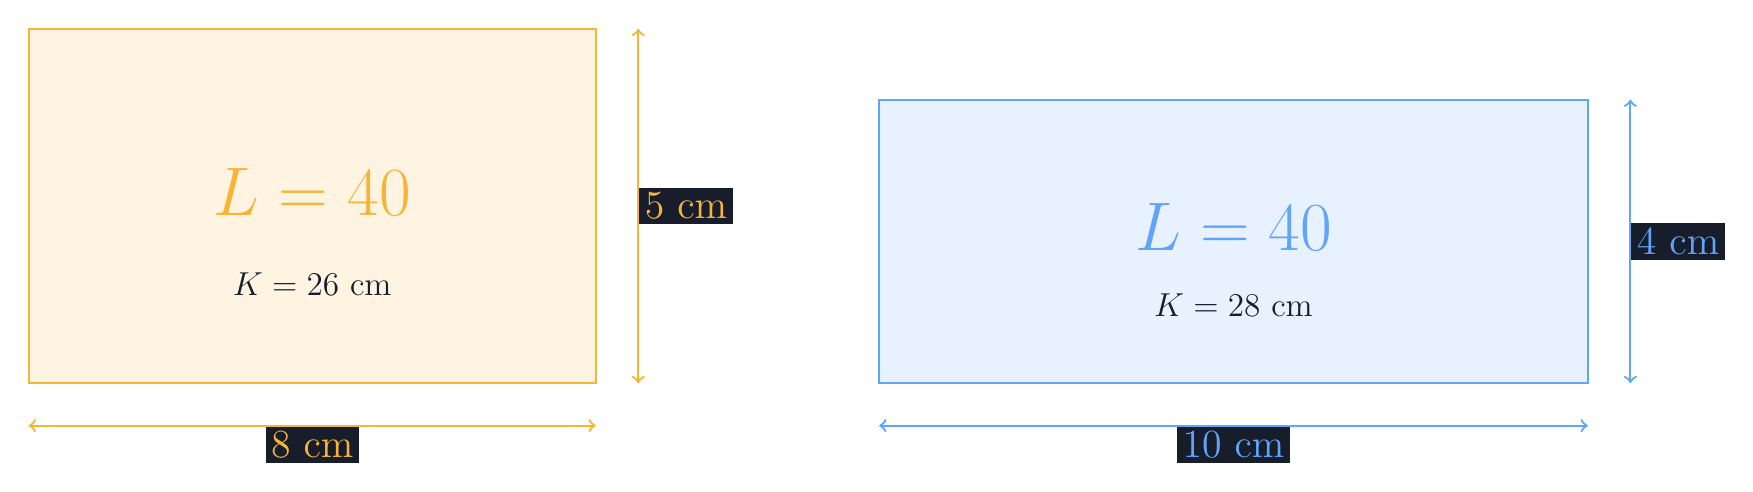
\begin{tikzpicture}[scale=0.9]
  % Persegi panjang P: 8 x 5
  \draw[thick,aksen,fill=aksen!15] (0,0) rectangle (8,5);
  \draw[aksen,thick,<->] (0,-0.6) -- (8,-0.6) node[midway,below,fill=bgcol,inner sep=2pt]{\Large 8 cm};
  \draw[aksen,thick,<->] (8.6,0) -- (8.6,5) node[midway,right,fill=bgcol,inner sep=2pt]{\Large 5 cm};
  \node[aksen] at (4,2.7) {\Huge $L = 40$};
  \node[bgcol] at (4,1.4) {\large $K = 26$ cm};

  % Persegi panjang Q: 10 x 4
  \begin{scope}[xshift=12cm]
    \draw[thick,biru,fill=biru!15] (0,0) rectangle (10,4);
    \draw[biru,thick,<->] (0,-0.6) -- (10,-0.6) node[midway,below,fill=bgcol,inner sep=2pt]{\Large 10 cm};
    \draw[biru,thick,<->] (10.6,0) -- (10.6,4) node[midway,right,fill=bgcol,inner sep=2pt]{\Large 4 cm};
    \node[biru] at (5,2.2) {\Huge $L = 40$};
    \node[bgcol] at (5,1.1) {\large $K = 28$ cm};
  \end{scope}
\end{tikzpicture}
\end{document}
